\documentclass{article}
\usepackage[utf8]{inputenc}
\usepackage{graphicx}
\usepackage{tikz}
\usepackage{listings}
\usepackage{xcolor}

\definecolor{codegreen}{rgb}{0,0.6,0}
\definecolor{codegray}{rgb}{0.5,0.5,0.5}
\definecolor{codepurple}{rgb}{0.58,0,0.82}
\definecolor{backcolour}{rgb}{0.95,0.95,0.92}

\lstdefinestyle{mystyle}{
    backgroundcolor=\color{backcolour},   
    commentstyle=\color{codegreen},
    keywordstyle=\color{magenta},
    numberstyle=\tiny\color{codegray},
    stringstyle=\color{codepurple},
    basicstyle=\ttfamily\footnotesize,
    breakatwhitespace=false,         
    breaklines=true,                 
    captionpos=b,                    
    keepspaces=true,                 
    numbers=left,                    
    numbersep=5pt,                  
    showspaces=false,                
    showstringspaces=false,
    showtabs=false,                  
    tabsize=2
}

\lstset{style=mystyle}
\renewcommand{\lstlistingname}{Algoritmo}

\title{Protocolo}
\author{Dueñas Jiménez Cristian Alexis\\Teoría de la computación}
\date{Octubre 2022}

\begin{document}

\maketitle
\section{Introducción}
El problema se nos plantea de la siguiente manera:
Debe de verificar si el protocolo está encendido o apagado y ejecutarse nuevamente si está encendido. El programa deberá determinar automáticamente en que momento detenerse. Generar $10^6$ cadenas binarias aleatoriamente de longitud 64. Posteriormente validar cada una de las cadenas con el AFD de imparidad.
\section{Marco Teórico}
Un\textbf{autómata finito determinista}, es la implementación de un autómata que sólo puede estar en un único estado después de leer cualquier secuencia de entradas. El término "determinista" hace referencia al hecho de que para cada entrada sólo existe uno y sólo un estado al que el autómata puede hacer la transición a partir de su estado actual.En palabras más simples, en un DFA(o AFD, por sus siglas en inglés y español respectivamente), sólo es posible seguir un camino por condición. 
Un Autómata Finito Determinista consta de:
\begin{enumerate}
    \item Un conjunto finito de estados, a menudo designado como $Q$.
    \item Un conjunto finito de símbolos de entrada, a menudo designado como $\Sigma$ (sigma).
    \item Una función de transición que toma como argumentos un estado y un símbolo de entrada y devuelve un estado. La función de transición se designa habitualmente como $\delta$ o $\Delta$ (delta).
    \item Un estado inicial, uno de los estados de $Q$.
    \item Un conjunto de estados finales o de aceptación $F$. El conjunto $F$ es un subconjunto de $Q$.
\end{enumerate}
La representación más sucinta de un AFD consiste en un listado de los cinco componentes anteriores. Normalmente, en las demostraciones, definiremos un AFD utilizando la notación de quíntupla siguiente:
$A= ( Q, \Sigma, \delta, q0, F )$

\begin{figure}[h!]
\centering
\includegraphics[width = 8cm]{dfa.PNG}
\caption{Representación gráfica de un DFA}
\end{figure}

Un \textbf{autómata finito no determinista}(NFA o AFN por sus siglas en inglés y español respectivamente), es el autómata finito que tiene transiciones vacías o que por cada símbolo desde un estado de origen se llega a más de un estado destino, es decir, es aquel que, a diferencia de los autómatas finitos deterministas, posee al menos un estado , tal que para un símbolo  del alfabeto, existe más de una transición posible. En palabras más simples, en un NFA tenemos varios caminos posibles dada una condición.
Un Autómata Finito No Determinista consta de:
\begin{enumerate}
    \item Un conjunto finito de estados, a menudo designado como $Q$.
    \item Un conjunto finito de símbolos de entrada, a menudo designado como $\Sigma$ (sigma).
    \item Una función de transición que toma como argumentos un estado y un símbolo de entrada y devuelve un estado. La función de transición se designa habitualmente como $\delta$ o $\Delta$ (delta).
    \item Un estado inicial, uno de los estados de $Q$.
    \item Un conjunto de estados finales o de aceptación $F$. El conjunto $F$ es un subconjunto de $Q$.
\end{enumerate}
\newpage
\section{Desarrollo}
En la implementación, primero planteamos un autómata que nos permita verificar si existe paridad en la cadena.

%DFA, NFA, DFA a NFA, grafos, código, ss's
\begin{center}
    \includegraphics[width = 10cm]{grafoProto.PNG}
    \caption{Representación gráfica del automata de paridad.}
    \newline
\end{center}
El programa básicamente sigue a ese autómata, y al llegar al estado final, determina que tiene paridad.

\begin{lstlisting}[language=Python, caption=Implementación de DFA]
import os
import sys
from functions import *

count = 0
iteration = 1
v1 = getRandomNumber(1)

if (iteration == 1) and (v1 == 0):
    print("El valor que se obtuvo fue 0. Protocolo cerrado.")
    sys.exit()

#Creamos los respectivos archivos
f1 = open("../PARCIAL 1/PROGRAMAS/Programa3/Version2/Outputs/stringBinary.txt", "w")
f2 = open("../PARCIAL 1/PROGRAMAS/Programa3/Version2/Outputs/parityBinary.txt", "w")
f3 = open("../PARCIAL 1/PROGRAMAS/Programa3/Version2/Outputs/notParityBinary.txt", "w")
f4 = open("../PARCIAL 1/PROGRAMAS/Programa3/Version2/Outputs/history.txt", "w")

#Generamos el bucle, que mantendrá activo el protocolo
while v1 == 1:
    print("Protocolo activo: " + os.linesep + "Veces que se ha activado: ")
    print(str(iteration))
    f1.write("Ciclo " + str(iteration) + os.linesep)
    f2.write("Cadenas del Ciclo " + str(iteration) + " con paridad: " + os.linesep)
    f3.write("Cadenas del Ciclo " + str(iteration) + " sin paridad: " + os.linesep)
    f4.write("Historial para el Ciclo " + str(iteration) + os.linesep)
    #Mandamos a llamar nuestra función que grafica el automata.
    if((v1 == 1) and (iteration == 1)):
        graphicMode()
    iteration+=1    #Incrementamos la iteración por cada bucle
    for x in range (0,1000000):   #Hacemos un for para generar el millón de cadenas binarias.
        rand = getRandomNumber(500000)   #Establecemos que se cree un número random
        binary = bin(rand)[2:]    #Lo convertimos a una cadena binaria
        f1.write(binary + ", ")      
        automata(binary, f2, f3, f4)     #Le mandamos la cadena binaria y los archivos para que pueda escribir sobre ellos.
    
    f1.write(os.linesep)
    f2.write(os.linesep)
    f3.write(os.linesep)
    f4.write(os.linesep)
    v1 = getRandomNumber(1) 
\end{lstlisting}

Este programa manda a llamar a una libreria, la cual generamos nosotros mismos, en esta librería viene la función que contiene el autómata, y a su vez grafica al mismo.

\begin{lstlisting}[language=Python, caption=Librería que contiene las funciones de nuestra clase principal]
import random
from graphics import *
from draws import *

def getRandomNumber(lim):
    randomNumber = random.randint(0,lim)
    return randomNumber

def graphicMode():
    window = GraphWin('Autómata de Paridad para cadenas Binarias', 900, 1500) 

    message = graphicText(window.getWidth()/2, 20, 'Autómata-Paridad Cadenas Binarias', 24, "black", "courier")
    message.setStyle("italic")
    message.draw(window)

    head0 = graphicCircle(300,280,35, "white", "purple", 3)
    head01 = graphicCircle(300,280,30, "white", "purple", 3)
    head1 = graphicCircle(450,410,35, "white", "purple", 3)
    head2 = graphicCircle(600,280,35, "white", "purple", 3)
    head3 = graphicCircle(450,150,35, "white", "purple", 3)

    state0 = graphicText(300,280,'q0',16,"black","arial")
    state1 = graphicText(450,410,'q1',16,"black","arial")
    state2 = graphicText(600,280,'q2',16,"black","arial")
    state3 = graphicText(450,150,'q3',16,"black","arial")

    t1 = graphicText(390, 230, '0', 13, "black", "arial")
    t2 = graphicText(350, 195, '0', 13, "black", "arial")
    t3 = graphicText(510, 230, '1', 13, "black", "arial")
    t4 = graphicText(550, 195, '1', 13, "black", "arial")
    t5 = graphicText(390, 330, '1', 13, "black", "arial")
    t6 = graphicText(350, 365, '1', 13, "black", "arial")
    t7 = graphicText(510, 330, '0', 13, "black", "arial")
    t8 = graphicText(550, 365, '0', 13, "black", "arial")

    lineinitial = graphicLine(265,280,200,280)
    line0a3 = graphicLine(415,155,310,245)
    line3a0 = graphicLine(330,265,430,180)
    line1a0 = graphicLine(310,315,415,400)
    line0a1 = graphicLine(435,380,330,295)
    line1a2 = graphicLine(590,315,485,400)
    line2a1 = graphicLine(465,380,570,295)
    line3a2 = graphicLine(570,265,470,180)
    line2a3 = graphicLine(485,155,590,245)

    #Automata Protocolo
    lineinit2 = graphicLine(315,540,235,540)
    head00 = graphicCircle(350, 540, 35, "white", "purple", 3)
    head10 = graphicCircle(550, 540, 35,  "white", "purple", 3)
    text0 = graphicText(275, 530, 'init', 14, "black", "arial")
    text1 = graphicText(350,540,'q0',16,"black","arial")
    text2 = graphicText(550,540,'q1',16,"black","arial")
    text3 = graphicText(450,500,'data',12,"black","arial")
    text4 = graphicText(450,580,'back',12,"black","arial")
    text5 = graphicText(650,540,'timeout',12,"black","arial")
    lineSecond = graphicLine(530,510,370,510)
    lineSecond1 = graphicLine(370,570,530,570)
    lineUlti = graphicLine(570,570,615,540)
    lineUlti2 = graphicLi(570,510,615,540)

    head0.draw(window)
    head01.draw(window)
    head1.draw(window)
    head2.draw(window)
    head3.draw(window)
    
    state0.draw(window)
    state1.draw(window)
    state2.draw(window)
    state3.draw(window)

    lineinitial.draw(window)
    line0a3.draw(window)
    line3a0.draw(window)
    line1a0.draw(window)
    line0a1.draw(window)
    line1a2.draw(window)
    line2a1.draw(window)
    line3a2.draw(window)
    line2a3.draw(window)

    t1.draw(window)
    t2.draw(window)
    t3.draw(window)
    t4.draw(window)
    t5.draw(window)
    t6.draw(window)
    t7.draw(window)
    t8.draw(window)

    #Dibujamos el automaa de protocolo
    lineinit2.draw(window)
    lineUlti.draw(window)
    lineUlti2.draw(window)
    head00.draw(window)
    head10.draw(window)
    text0.draw(window)
    text1.draw(window)
    text2.draw(window)
    text3.draw(window)
    text4.draw(window)
    text5.draw(window)
    lineSecond.draw(window)
    lineSecond1.draw(window)

    window.getMouse()
    window.close()

def automata(cadena,aceptar,rechazar,hist):
    estado = 0
    for char in cadena:
        if estado == 0:
            if char == "0":
                estado = 1
            if char == "1":
                estado = 3
            hist.write("(q0,\""+char+"\",q"+str(estado)+")\n")
            continue

        if estado == 1:
            if char == "0":
                estado = 0
            if char == "1":
                estado = 2
            hist.write("(q1,\""+char+"\",q"+str(estado)+")\n")
            continue

        if estado == 2:
            if char == "0":
                estado = 3
            if char == "1":
                estado = 1
            hist.write("(q2,\""+char+"\",q"+str(estado)+")\n")
            continue

        if estado == 3:
            if char == "0":
                estado = 2
            if char == "1":
                estado = 0
            hist.write("(q3,\""+char+"\",q"+str(estado)+")\n")
            continue
    hist.write("\n")
    if estado == 0:
        aceptar.write(cadena+"  \n")
    else: 
        rechazar.write(cadena+"  \n")

\end{lstlisting}

A su vez, este se conecta a otra librería, la cual se encarga de asignarle las propiedades a cada elemento, reduciendo un poco el código.

\begin{lstlisting}[language=Python, caption=Librería que contiene las propiedades de los elementos.]

from graphics import *

def graphicCircle(x, y, r, color, border, width):
    head = Circle(Point(x,y), r)
    head.setFill(color)
    head.setOutline(border)
    head.setWidth(width)
    return head

def graphicText(x,y,cadena, width, color, font):
    label = Text(Point(x,y), cadena)
    label.setFill(color)
    label.setFace(font)
    label.setSize(width)
    return label

def graphicLine(w,x,y,z):
    line = Line(Point(w,x), Point(y,z))
    line.setWidth(3)
    line.setArrow("first")
    line.setFill("black")
    return line

def graphicLi(w,x,y,z):
    line = Line(Point(w,x), Point(y,z))
    line.setWidth(3)
    line.setFill("black")
    return line

\end{lstlisting}

\begin{center}
    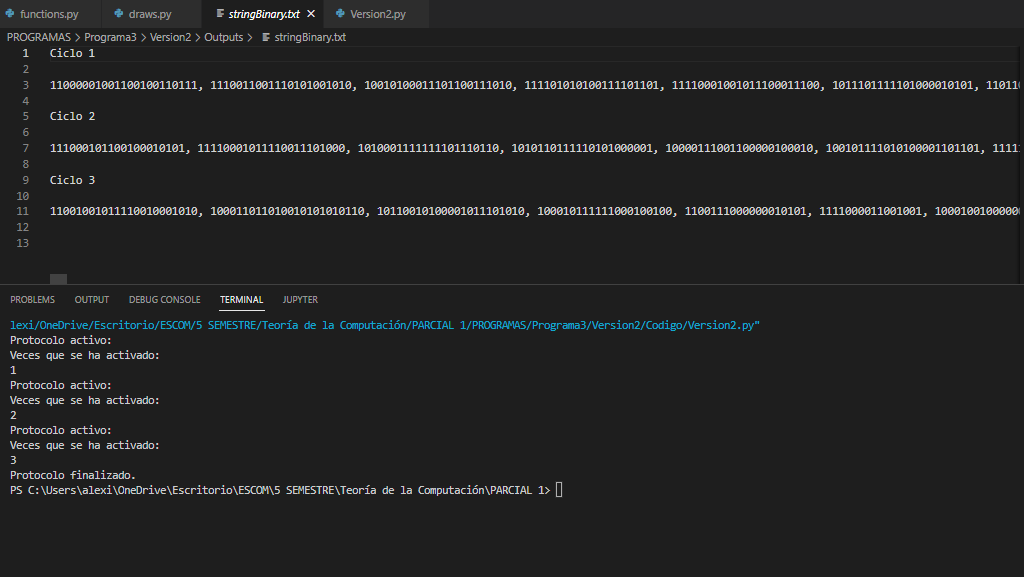
\includegraphics[width = 12cm]{test1.PNG}
    \newline\newline
    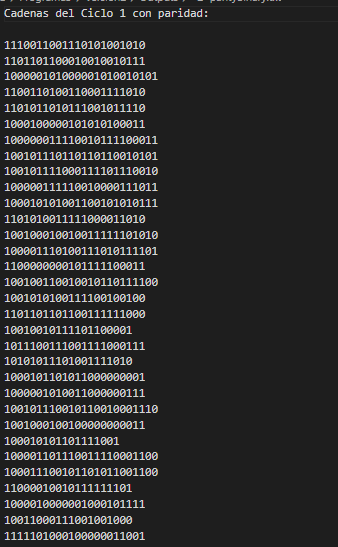
\includegraphics[width = 12cm]{Paridad.PNG}
    \newline\newline
    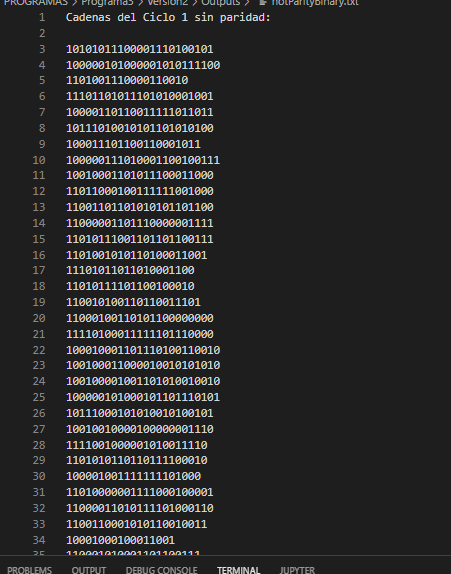
\includegraphics[width = 12cm]{NotParidad.PNG}
    \newline\newline
    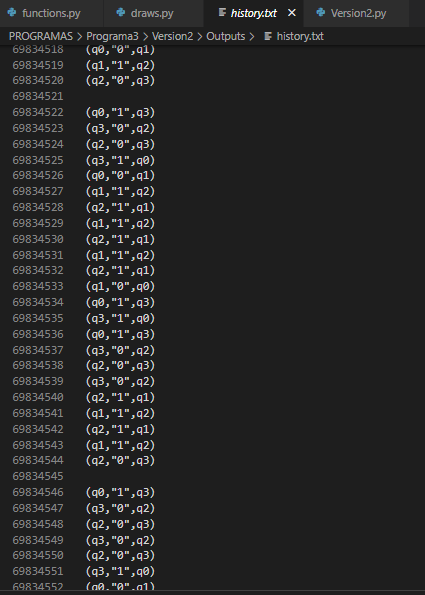
\includegraphics[width = 12cm]{history.PNG}
    \newline\newline
    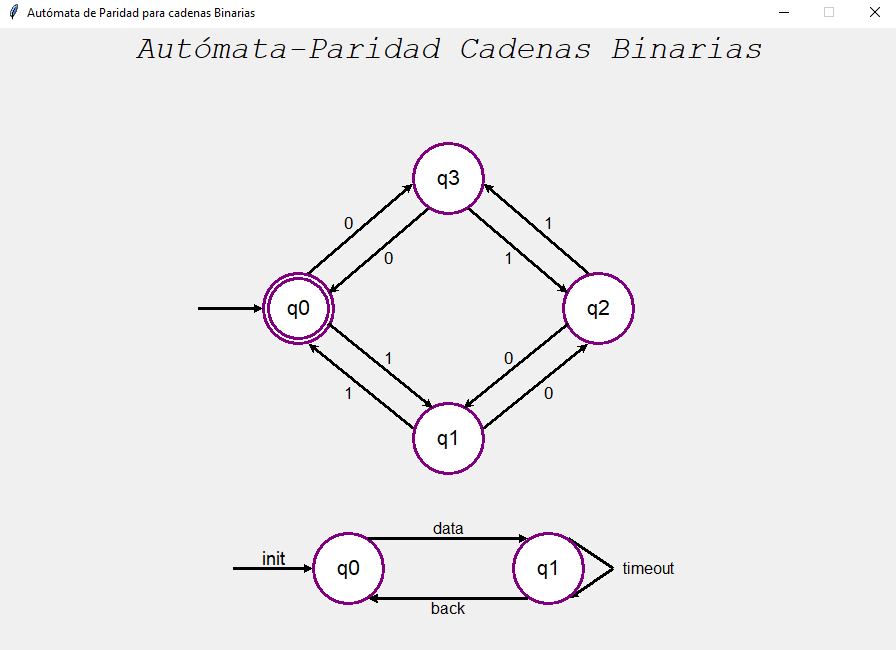
\includegraphics[width = 12cm]{graphic.PNG}
\end{center}
\newpage

\section{Conclusión}
Gracias a este programa, fuimos capaces de mejorar y comprender al completo tanto los DFA's. Me pareció un ejercicio bastante sencillo, así como una buena introducción al tema de autómatas de estados finitos. Sus aplicaciones pueden ir desde lo más básico, como este ejercicio, hasta cosas enormes como redes neuronales. Estos ejercicios nos ayudan a comprender el lenguaje y entendimiento de las computadoras.

\begin{thebibliography}{}
    \bibitem
    ¿Como se transforma un AFN en un AFD? (s. f.). Teoría de Automatas y Lenguajes Formales. Recuperado 5 de junio de 2022, de http://repositori.uji.es/xmlui/bitstream/handle/10234/5875/bolAuto1.pdf?sequence=1
    
    
\end{thebibliography}

\end{document}

